\documentclass[12pt]{article}

\usepackage{parskip}
\usepackage{listings}
\usepackage[charter]{mathdesign}
\usepackage{nimbusmono}
\usepackage{hyperref}
\usepackage[margin=1in]{geometry}
\usepackage{graphicx}

\lstset{
    language=C,
    basicstyle=\small\ttfamily,
    xleftmargin=1em
}

\author{Jesse op den Brouw\thanks{Please mail me at: \href{mailto:J.E.J.opdenBrouw@hhs.nl}{J.E.J.opdenBrouw@hhs.nl}}\\The Hague University of Applied Sciences\\(THUAS)}
\title{Graphic LCD Routines for Velleman VMA412 with ILI9341 Controller}
\date{\today}


\begin{document}
\maketitle

\vfill
{\small\leftskip=1em\rightskip=1em
The Velleman VM412 is an Arduino Uno/Mega compatible 2.8" color Graphic LCD with 320x240 pixels controlled by an ILI9431 graphic controller.
The ILI9431 is connected using an 8-bit 8080 interface to the board. More information can be found via
\url{https://www.velleman.eu/products/view/?id=435582}.

The software is written in C and consists of two driver files and one C test file.

Functions include plotting a pixel, rectangles, circles, arcs, printing strings and filling an object.
It also has primitive console based printing routines.

The software uses 18-bit colors where each color has 6 bits used.

The software is tested using a STM32F446 Nucleo board and STMCubeIDE version 1.3.1.

}
\vfill

\newpage
\tableofcontents


\newpage
\section{Mouting the VMA412}
The Velleman VM412 is an Arduino Uno/Mega compatible 2.8" color Graphic LCD with 320x240 pixels controlled by an ILI9431 graphic controller.
The VMA412 has an Arduino Uno compatible connection and can be connected to numerous STM32F Nucleo boards.
Place the VM412 board as instructed. See the picture below for a visual inspection.

\begin{figure}[!ht]
\centering
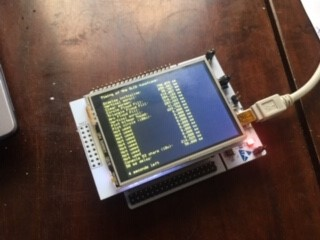
\includegraphics[scale=1]{setup_small}
test
\end{figure}


\section{Creating a project}
With STM32CubeIde, create a standard project for a STM32F446RE microcontroller. There is no need to
create a board project, just a chip project. 

After creating a project, just place the three files in the appropriate folders. There are three files;

\begin{lstlisting}
glcd_ili9341_stm32.h   -- place in Core/Inc, definitions, typedefs etc
glcd_ili9341_stm32.c   -- place in Core/Src, functions to call
main.c                 -- place in Core/Src, demo using functions
\end{lstlisting}

\section{Running the demo}
Place the files in the appropriate folders and start compilation using \texttt{Project}$\rightarrow$\texttt{Build Project}.
Then start the the demo using \texttt{Run}$\rightarrow$\texttt{Run}. At the end of the demo, there will be a list of running times for selected graphic functions as can be seen in the figure above.

\section{Color system}
The GLCD is set up to use the 18-bit color specification. This means that colors are specified with unsigned 32 bits. The specification as follows:

Bits 31-24: should be kept at 0.\\
Bits 23-16: red -- only upper 6 bits are used\\
Bits 15-8: green -- only upper 6 bits are used\\
Bits 7-0: blue -- only upper 6 bits are used

\textbf{Note:} The 16 bit color specification in \textbf{NOT} supported.

Please note that although 8 bits per color can be specified, only the upper 6 bits of each color are used, since the display uses 18 bits of color infomation. The lower 2 bits are ignored.

The color is specified using the the type \lstinline|glcd_color_t|.

\subsection{Predefined colors}
There are some predefines colors:

\begin{lstlisting}
#define GLCD_COLOR_BLACK   (0x000000)
#define GLCD_COLOR_BLUE    (0x0000ff)
#define GLCD_COLOR_GREEN   (0x00ff00)
#define GLCD_COLOR_CYAN    (0x00ffff)
#define GLCD_COLOR_RED     (0xff0000)
#define GLCD_COLOR_MAGENTA (0xff00ff)
#define GLCD_COLOR_YELLOW  (0xffff00)
#define GLCD_COLOR_WHITE   (0xffffff)

#define GLCD_COLOR_GREY50  (0x7f7f7f)

/* THUAS default color */
#define GLCD_COLOR_THUASGREEN ((158<<16)|(167<<8)|0)
\end{lstlisting}

\subsection{Using your own color}
To use your own color, please use the color type \lstinline|glcd_color_t|:

\begin{lstlisting}
glcd_color_t SkyBlue2 = (126<<16)|(192<<8)|238
\end{lstlisting}

\section{X and Y coordinates}
The X and Y coordinates use type \lstinline|uint16_t| for their values. The screen is set up in landscape where \lstinline|X| is between 0 and 319 and \lstinline|y| is between 0 and 239. Point (0,0) is in the upper left corner.



\section{Initialisation}
First you have to set up the clock system used by the STM32F microcontroller. If you use the onboard (but external) clock generator, make sure that the value of \lstinline|HSE_VALUE| is set to the correct frequency. In the case of the Nucleo board it is 8000000 (8 MHz). If you use the internal HSI (\lstinline|HSIVALUE|), the frequency is 16 MHz by default. Best is to set up the clock speed to the maximum frequency allowed by the microcontroller.

Initialise the graphic VMA412 and graphic routines by calling the \lstinline|glcd_init()| routine. After calling that routine the display is initialised and ready for use.

\subsection{Initialize display}
This function must be called after the clock system is set up and before using any other GLCD functions. The function prototype is:
\begin{lstlisting}
void glcd_init(void);
\end{lstlisting}

Note: call this function \textbf{after} the clock system is set up.

\subsection{Setting the read/write delay}
\textbf{Note:} use with care.\\
Sets the delay for read/write actions. There is no need to call this function as the correct timing is calculated according to the system clock speed after the clock system is set up. \lstinline|delay| must be greater than 0. The function prototype is:
\begin{lstlisting}
void glcd_set_write_pulse_delay(uint32_t delay);
\end{lstlisting}


\section{Low level functions}
There are a number of low level functions. They are normally not needed.

\subsection{Reading data from the display}
Te read data from the display, use the function \lstinline|glcd_read_terminate|. Reading is explictly terminated. The function prototype is:

\begin{lstlisting}
void glcd_read_terminate(uint16_t cmd,            // The command
                         uint16_t amount,         // Amount of data
                         glcd_buffer_t data[]);   // The buffer
\end{lstlisting}

\subsection{Writing data to the display}
Writes data to the display, no explicit terminate:
\begin{lstlisting}
void glcd_write(uint16_t cmd,                     // The command
                uint16_t amount,                  // Amount of data
                const glcd_buffer_t data[]);      // The buffer
\end{lstlisting}

\subsection{(Explicit) terminating a write}

Terminates a write:
\begin{lstlisting}
void gcld_terminate_write(void);
\end{lstlisting}

\subsection{Changing the buffer type}
The low level routines use an internal buffer. The buffer is of type \lstinline|glcd_buffer_t|. This normally set to an unsigned 16-bit size. This size can be changed:

Set to \lstinline|uint8_t| for minimal resources\\
Set to \lstinline|uint16_t| for best speed\\
Set to \lstinline|uint32_t| for maximum capacity (not recommended)
 
\section{High level commands}

\subsection{Delay}

To delay your applications (in milliseconds), use :
\begin{lstlisting}
void glcd_delay_ms(uint32_t delay);
\end{lstlisting}

\subsection{Rotating the screen}
To set the rotation of the screen, use:
\begin{lstlisting}
void glcd_setrotation(glcd_rotation_t rot);
\end{lstlisting}

Where \lstinline|rot| is one of:

\begin{lstlisting}
GLCD_SCREEN_ROT0           // Standard landscape, default
GLCD_SCREEN_ROT90          // Rotate 90 degrees
GLCD_SCREEN_ROT180         // Rotate 180 degrees
GLCD_SCREEN_ROT270         // Rotate 270 degrees
\end{lstlisting}

\subsection{Clear the screen}
To clear the screen with a color, use:
\begin{lstlisting}
void glcd_cls(glcd_color_t color);
\end{lstlisting}

\subsection{Plot a pixel}
To plot a pixel, use:
\begin{lstlisting}
void glcd_plotpixel(uint16_t x,           // x coordinate
                    uint16_t y,           // y coordinate
                    glcd_color_t color);  // color
\end{lstlisting}

\subsection{Read a pixel}
To read a pixel (getting color information), use:

\begin{lstlisting}
glcd_color_t glcd_readpixel(uint16_t x,   // x coordinate
                            uint16_t y);  // y coordinate
\end{lstlisting}

\subsection{Plot a horizontal line}
To plot a horizontal line (fast), use:
\begin{lstlisting}
void glcd_plothorizontalline(uint16_t x,           // x coordinate
                             uint16_t y,           // y coordinate
                             uint16_t w,           // width
                             glcd_color_t color);  // color
\end{lstlisting}


\subsection{Plot a vertical line}
To plot a vertical line (fast), use:
\begin{lstlisting}
void glcd_plotverticalline(uint16_t x              // x coordinate
                           uint16_t y,             // y coordinate
                           uint16_t h,             // height
                           glcd_color_t color);    // color
\end{lstlisting}

\subsection{Plot a line with any angle}
To plot a line with any angle and length, use:
\begin{lstlisting}
void glcd_plotline(uint16_t x0,            // x start point
                   uint16_t y0,            // y start point
                   uint16_t x1,            // z end point
                   uint16_t y1,            // y end point
                   glcd_color_t color);    // color
\end{lstlisting}

\subsection{Plot a character using buildin font}
To plot a character using the buildin fond (5x8), use:
\begin{lstlisting}
void glcd_plotchar(uint16_t x,             // x coordinate
                   uint16_t y,             // y coordinate
                   uint8_t c,              // character (0-255)
                   glcd_color_t color,     // color
                   glcd_color_t bg);       // background color
\end{lstlisting}

Note: character is one of 0 -- 255 (no special C treatment)\\
Note: if \texttt{color} is \texttt{bg} then pixels having background color are not printed! 

\subsection{Plot a string using buildin font}
To plot a string using the buildin font, use:
\begin{lstlisting}
void glcd_plotstring(uint16_t x,                  // x coordinate
                     uint16_t y,                  // y coordinate
                     char str[],                  // the string
                     glcd_color_t color,          // color
                     glcd_color_t bg,             // background color
                     glcd_spacing_t spacing);     // spacing
\end{lstlisting}

Note: a \texttt{'\textbackslash 0'} terminates a string (as in C)\\
Note: is \texttt{color} is \texttt{bg} then pixels having background color are not printed!\\
Note: \texttt{spacing} is one of:
\begin{lstlisting}
GLCD_STRING_CONDENSED  // zero pixels apart
GLCD_STRING_NORMAL     // one pixel apart
GLCD_STRING_WIDE       // two pixels apart
\end{lstlisting}

\subsection{Plot a rectangle}
To plot a rectangle, use:
\begin{lstlisting}
void glcd_plotrect(uint16_t x,             // x coordinate
                   uint16_t y,             // y coordinate
                   uint16_t w,             // width
                   uint16_t h,             // height
                   glcd_color_t color);    // color
\end{lstlisting}

\subsection{Plot a filled recangle}
To plot a filled rectangle, use:
\begin{lstlisting}
void glcd_plotrectfill(uint16_t x,            // x coordinate
                       uint16_t y,            // y coordinate
                       uint16_t w,            // width
                       uint16_t h,            // height
                       glcd_color_t color);   // color
\end{lstlisting}

\subsection{Plot a circle}
To plot a circle, use:
\begin{lstlisting}
void glcd_plotcircle(uint16_t x0,             // center x coordinate
                     uint16_t y0,             // center y coordinate
                     uint16_t r,              // radius
                     glcd_color_t color);     // color
\end{lstlisting}

\subsection{Plot an arc}
To plot an arc, use:
\begin{lstlisting}
void glcd_plotarc(uint16_t xc,                // center x coordinate
                  uint16_t yc,                // center y coordinate
                  uint16_t r,                 // radius
                  float start,                // start angle in degrees
                  float stop,                 // stop angle in degrees
                  glcd_color_t color);        // color
\end{lstlisting}

Note: this function is only available if \lstinline|GLCD_USE_ARC| is defined.\\
Note: this function uses \lstinline|sinf| and \lstinline|cosf| math functions.

\subsection{Plot a 2-color bitmap}
To plot a 2-color bitmap, use:
\begin{lstlisting}
void glcd_plotbitmap(uint16_t x,              // x coordinate
                     uint16_t y,              // y coordinate
                     const uint8_t bitmap[],  // the bitmap, see note
                     uint16_t w,              // width
                     uint16_t h,              // height
                     glcd_color_t color,      // color
                     glcd_color_t bg);        // background color
\end{lstlisting}

Note: \lstinline|bitmap| consists of bytes (\lstinline|uint8_t|). A 1 in a byte is converted to \lstinline|color|, a 0 in a byte is converted to \lstinline|bg|.

\subsection{Display inversion}
Sets the display inversion (or not):
\begin{lstlisting}
void glcd_inversion(glcd_display_inversion_t what);
\end{lstlisting}

Note: \lstinline|what| is one of:
\begin{lstlisting}
GLCD_DISPLAY_INVERSION_OFF
GLCD_DISPLAY_INVERSION_ON
\end{lstlisting}

\subsection{Display idle}
Set the display to idle (or not):
\begin{lstlisting}
void glcd_idle(glcd_display_idle_t what);
\end{lstlisting}

Note: \lstinline|what| is one of:

\begin{lstlisting}
GLCD_DISPLAY_IDLE_OFF
GLCD_DISPLAY_IDLE_ON
\end{lstlisting}

\subsection{Display ON or OFF}
Sets the display on or off:
\begin{lstlisting}
void glcd_display(glcd_display_t what);
\end{lstlisting}

Note: \lstinline|what| is one of

\begin{lstlisting}
GLCD_DISPLAY_OFF
GLCD_DISPLAY_ON
\end{lstlisting}

\subsection{Flood fill an object}
Flood fill and object using a stack based approach:
\begin{lstlisting}
void glcd_floodfill(uint16_t xs,                 // x start point
                    uint16_t ys,                 // y start point
                    glcd_color_t fillColor,      // color for pixel == 1
                    glcd_color_t defaultColor);  // color for pixel == 0
\end{lstlisting}

Note: this function is only available if \lstinline|GLCD_USE_FLOOD_FILL| is defined.\\
Note: set \lstinline|GLCD_STACK_SIZE| to an appropiate value.\\
Note: if you have problems filling an object increase the value of \lstinline|GLCD_STACK_SIZE|.

\subsection{Scroll the display vertical}
To scroll the display vertical a number of lines, use:
\begin{lstlisting}
void glcd_scrollvertical(uint16_t lines);   // number of lines to scroll
\end{lstlisting}

Note: this is a software based scroll, could be slow.

\subsection{Console based character printing}
To use a simple console based character printing, use:
\begin{lstlisting}
void glcd_putchar(char c);
\end{lstlisting}

Note: characters are printed in yellow, background is black\\
Note: \lstinline|\f| (form feed) clears the screen\\
Note: \lstinline|\n| returns and goes to the next line\\
Note: \lstinline|\r| return to the beginning of the line\\
Note: \lstinline|\b| erases last character and goes one character back\\
Note: all other characters are printed using the internal font\\
Note: if a character ``falls off'' the display, line wrap will be used, may cause a vertical shift

\subsection{Console based string printing}
To use a simple console based string printing use:
\begin{lstlisting}
void glcd_printconsole(char str[]);
\end{lstlisting}

Note: \lstinline|str| is null-terminated as in C.\\
Note: characters are printed in yellow, background is black\\
Note: \lstinline|\f| (form feed) clears the screen\\
Note: \lstinline|\n| returns and goes to the next line\\
Note: \lstinline|\r| return to the beginning of the line\\
Note: \lstinline|\b| erases last character and goes one character back\\
Note: all other characters are printed using the internal font\\
Note: if a character ``falls off'' the display, line wrap will be used, may cause a vertical shift



\end{document}
